

\documentclass[14pt]{article}
\usepackage{listings}
\usepackage{color}
\usepackage{graphicx}
\usepackage{setspace}

\definecolor{dkgreen}{rgb}{0,0.6,0}
\definecolor{gray}{rgb}{0.5,0.5,0.5}
\definecolor{mauve}{rgb}{0.58,0,0.82}

\lstset{frame=tb,
  language=C,
  aboveskip=3mm,
  belowskip=3mm,
  showstringspaces=false,
  columns=flexible,
  basicstyle={\small\ttfamily},
  numbers=none,
  numberstyle=\tiny\color{gray},
  keywordstyle=\color{blue},
  commentstyle=\color{dkgreen},
  stringstyle=\color{mauve},
  breaklines=true,
  breakatwhitespace=true
  tabsize=3
}

\begin{document}
\title{\huge NxN queens problem}
\date{\today}
\maketitle
\begin{center}
\vspace{30 mm}

\title{\huge Student: Alexe Octavian-Alexandru}
\\\vspace{10 mm}
\title{\huge Computers and Information Technology}
\\\vspace{10 mm}
\title{\huge Group C.R. 1.1 A}
\\\vspace{10 mm}
\title{\huge 1st Year}
\date{}
\maketitle

\newpage
\section*{Introduction}
\vspace{20 mm}
Backtracking is a general algorithmic technique that considers searching every possible combination in order to solve an optimization problem. Backtracking is also known as depth-first search or branch and bound. By inserting more knowledge of the problem, the search tree can be pruned to avoid considering cases that don't look promising. While backtracking is useful for hard problems to which we do not know more efficient solutions, it is a poor solution for the everyday problems that other techniques are much better at solving.
\\
Backtracking reduces the search space since we no longer have to follow down any paths we know are invalid. This is called pruning. We must be able to test partial solutions: for example, we can’t find a global optimum using backtracking, since we have no idea if the solution we’re currently on can lead to it or not. But we can, for example, solve Sudoku using backtracking. We can know immediately if our solution so far is invalid by testing if two of the same number appear in the same row, column, or square.



\newpage
\end{center}
\section*{Problem statement}
\textbf{\textit{NxN Queens}}
\\
Implement two different algorithms to solve the N Queens problem on a N x N chess board, e.g., based on Backtracking and Dynamic Programming.
\\
\begin{center}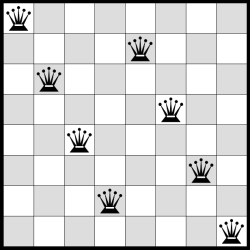
\includegraphics[height=3.5in, width = 3.5in]{8-queens-config.png}
\end{center}



\newpage
\section*{Pseudocode}
\textbf{Backtracking altgorithm}
\\
The idea is to place queens one by one in different columns, starting from the leftmost column. When we place a queen in a column, we check for clashes with already placed queens. In the current column, if we find a row for which there is no clash, we mark this row and column as part of the solution. If we do not find such a row due to clashes then we backtrack and return false.
\\
We will use functions for each operation required by the application, with integer parameters, which will be called by the main program.
\\
Here are the functions employed by the program:
\begin{lstlisting}
int main()
1.  read N
2.  print (" - N Queens Problem Using Backtracking -")
3.  print ("Enter number of Queens:")
4.	queen (1, N)
5.	print ("\n")
6.	return 0;
\end{lstlisting}
\begin{lstlisting}
int place(int row, int column)
1.	int i
2.	for i <- 1 to row-1
3.          if( board[i] == column)
4.	            return 0
5.          else
6.		        if ( |board[i]-column| == (i-row))
7.		            return 0
8.	return 1
\end{lstlisting}
\begin{lstlisting}
void printing(int n)
1.	int i
2.	int j
3.		for i <- 1  to n
4.			print i;
5.	    for i <- 1 to n
6.              print i;
7.          for j <- 1 to n
8.              if ( board[i] == j)
9.                  print("Q")
10.             else
11.                 print("-")
\end{lstlisting}
\begin{lstlisting}
void queen(int row, int n)
1.  int column;
2.		for column <- 1 to n do
3.          if( place(row, column) )
4.				board[row] = column
5.                  if (row == n)
6.                      printing (n)
7.                  else
8.                      queen(row+1 , n)
\end{lstlisting}



\newpage
\section*{Application design}
\vspace{10 mm}
The library contains the header \textbf{\textit{functions.h}} which has all the function prototypes to compute the required operations. These are all of them:
\\---void print(int n)
\\---int place(int row, int column)
\\---void queen(int row, int n)
\\\vspace{3 mm}
\\Function print(int n) is used to display problem solutions. Where the queen can be placed the function will put "Q" and where it can not be placed will put "-". 
\\\vspace{3 mm}
\\ Function place(int row, int column) is a function to check if the cell (row,column) is under attack by any other queen or not.Just checking if there is any other queen in the row or column. Then we are checking if there is any queen on the diagonal cells of the cell (row,column) or not.
\\\vspace{2 mm}
\\Function queen(int row, int n) is checking for proper positioning of queen.
 We are re looking for a position for our queen on the row "row". If there is a valid position,the queen it is placed, then call the function recursively: "queen(row+1,n)".
If a position isn’t found in this call the program will abandon that solution, and go back to where it was before. There, it will check again for the next value of column, and if the position is valid, it is then going to try again for row + 1, until there is a valid solution there. When it finds one, it is going to call queen() again, with row + 1.
 \textbf{\textit{2}}.


\newpage
\section*{Source Code}
\begin{lstlisting}
//-----------------------------functions.h-------------------------------

void print(int n);
int place(int row,int column);
void queen(int row,int n);
\end{lstlisting}

\begin{lstlisting}
//-----------------------------main.c-------------------------------

#include <stdio.h>
#include <stdlib.h>
#include "functions.h"



int main()
{
 int n;
 printf(" - N Queens Problem Using Backtracking -");
 printf("\n\nEnter number of Queens:");
 scanf("%d",&n);
 queen(1,n);
 printf("\n");
 system("pause");
 return 0;
}

\end{lstlisting}
\begin{lstlisting}



//---------------------------------place.c--------------------------------


#include "functions.h"
int board[20],count;

/*funtion to check conflicts
If no conflict for desired postion returns 1 otherwise returns 0*/
int place(int row,int column)
{
 int i;
 for(i=1;i<=row-1;i++)
 {
  //checking column and digonal conflicts
  if(board[i] == column)
   return 0;
  else
   if(abs(board[i]-column) == abs(i-row))
    return 0;
 }

 return 1; //no conflicts
}
\end{lstlisting}
\begin{lstlisting}



//-------------------------------print.c------------------------------

#include "functions.h"
int board[20],count;
//function for printing the solution
void print(int n)
{
 int i,j;
 printf("\n\nSolution %d:\n\n",count++);

 for( i=1; i<=n; i++ )
  printf("\t%d",i);

 for( i=1; i<=n; i++ )
 {
  printf("\n\n%d",i);
  for( j=1; j<=n; j++) //for nxn board
  {
   if(board[i] == j)
    printf("\tQ"); //queen at i,j position
   else
    printf("\t-"); //empty slot
  }
 }
}
\end{lstlisting}
\begin{lstlisting}


//---------------------------queen.c-------------------------------

#include "functions.h"
int board[20],count;
//function to check for proper positioning of queen
void queen(int row,int n)
{
 int column;
 for( column=1; column<=n; column++ )
 {
  if(place(row, column))
  {
   board[row] = column; //no conflicts so place queen
   if(row==n) //dead end
    print(n); //printing the board configuration
   else //try queen with next position
    queen(row+1,n);
  }
 }
}



\end{lstlisting}

\newpage
\section*{Experiments and results}
\begin{lstlisting}
Number of Queens: 6
Solution 0
    1   2   3   4   5   6
1   -   Q   -   -   -   -

2   -   -   -   Q   -   -

3   -   -   -   -   -   Q

4   Q   -   -   -   -   -

5   -   -   Q   -   -   -

6   -   -   -   -   Q   -   
Solution 1
    1   2   3   4   5   6
1   -   -   Q   -   -   -

2   -   -   -   -   -   Q

3   -   Q   -   -   -   -

4   -   -   -   -   Q   -

5   Q   -   -   -   -   -

6   -   -   -   Q   -   -
Solution 2:
    1   2   3   4   5   6
1   -   -   -   Q   -   -

2   Q   -   -   -   -   -

3   -   -   -   -   Q   -

4   -   Q   -   -   -   -

5   -   -   -   -   -   Q

6   -   -   Q   -   -   -
Solution 3:
    1   2   3   4   5   6
1   -   -   -   -   Q   -

2   -   -   Q   -   -   -

3   Q   -   -   -   -   -

4   -   -   -   -   -   Q

5   -   -   -   Q   -   -

6   -   Q   -   -   -   -


\end{lstlisting}


\newpage
\section*{Conclusions}
\vspace{10 mm}
By working on this project, I gained experience in using the Backtracking technique and I also managed to understand it. 
\\\vspace{10mm}
\section*{References}
\\
1)https://www.geeksforgeeks.org/
\\
\\\vspace{6mm}
\\
2)https://www.codesdope.com
\\
\\\vspace{6mm}
\\
5)http://www.sharelatex.com


\end{document}
